\documentclass{article}

\newcommand{\myhighlight}[1]{\textcolor{blue}{#1}}

% The draft follows the supplied NeurIPS-style template when the local style
% file exists, and falls back to a standard preprint layout in this workspace.
\IfFileExists{neurips_2026.sty}{%
  \usepackage[preprint]{neurips_2026}
}{%
  \usepackage[margin=1in]{geometry}
  \usepackage[numbers,sort&compress]{natbib}

}
\usepackage{needspace}
\usepackage{caption}
\usepackage{float}
\usepackage[utf8]{inputenc}
\usepackage[T1]{fontenc}
\usepackage{hyperref}
\usepackage{url}
\usepackage{booktabs}
\usepackage{amsfonts}
\usepackage{amsmath}
\usepackage{nicefrac}
\usepackage{microtype}
\usepackage[table]{xcolor}
\usepackage{enumitem}
\usepackage{tabularx}
\usepackage{array}
\usepackage{graphicx}
\usepackage{booktabs}
\usepackage{tabularx}
\usepackage{array}


\usepackage{tikz}
\usetikzlibrary{arrows.meta, positioning}
\newcolumntype{P}[1]{>{\centering\arraybackslash}p{#1}}
\usepackage{mathtools}
\usepackage{amsthm}
\theoremstyle{plain}
% \newtheorem{findings}{Findings}
\newtheorem{desideratum}{Desideratum}
\renewcommand{\thedesideratum}{\Roman{desideratum}}



\hypersetup{
  colorlinks=true,
  linkcolor=blue,
  citecolor=blue,
  urlcolor=blue
}

% \title{A Fault-Tolerant Hierarchical Multi-Agent Protocol for Public-Good Task Production}



\title{\textit{Share Your Tokens!}  A  Community Protocol for Composing Distributed Tokens  for   ``Intelligent'' Tasks}
% \title{Shared Token Economics:  A Protocol for Leveraging Local Tokens  for  Distributed ``Intelligent'' Tasks}
 % Verifiable and Scalable
% \author{Anonymous Author(s)}

\usepackage{authblk}
\author[1$\dagger$]{\textbf{Hongzhan Tu}}
\author[1$\dagger$]{\textbf{Zhizhou  Wang}}
\author[1,2*]{\textbf{Yan Hu}}
\author[1,2,3,4*]{\textbf{Benyou Wang}}
\affil[1]{The Chinese University of Hong Kong, Shenzhen, China}
\affil[2]{National Health Data Institute (Shenzhen),}
\affil[3]{Shenzhen Loop Area Institute}
\affil[4]{Shenzhen Research Institute of Big Data, Shenzhen, China}
% \affil[4]{Platform and Content Group, Tencent, China}
% \affil[5]{Halmstad University, Halmstad, Sweden}
\affil[*]{{huyan,wangbenyou@cuhk.edu.cn}}
\affil[-]{\url{https://tokenmosaic.github.io/}}
\begin{document}


% https://github.com/BriasedTu/TokenShare


\maketitle

\begin{abstract}
Large-scale public-good tasks, such as scientific computation, low-resource language documentation, and multi-source data annotation, increasingly require not only generation but also decomposition, verification, revision, and accountable integration. Modern AI systems suggest that useful outputs can often be obtained by spending sufficient tokens; however, the required token, compute, and human-execution resources may exceed the capacity of any single user or organization. Meanwhile, many personal devices, local GPUs, cloud credits, tool-execution environments, and human annotators remain under-utilized.

This paper proposes TokenMosaic, a protocol for aggregating idle tokens and heterogeneous execution capacity into useful, verifiable work. TokenMosaic represents a large task as a recursively decomposable task tree or DAG, assigns atomic units to distributed clients, supports local and server-side verification, reassigns failed tasks, recursively merges accepted outputs, and records contributions through a ledger. Unlike proof-of-work systems that coordinate untrusted participants around artificial computation, TokenMosaic focuses on useful computation with real public-good value. We outline the protocol design, fault-tolerance mechanisms, incentive settlement, and evaluation plan, aiming to measure not only final output quality but also reliability, provenance, recoverability, cost, and verifiability.
\end{abstract}

\section{Introduction}


The infinite monkey theorem offers a useful metaphor for modern AI computation: with enough attempts, even highly complex outputs can in principle be produced. In today’s AI systems, these “attempts” are largely mediated by tokens. For many tasks, better outputs can be achieved by spending more tokens on planning, decomposition, generation, tool use, verification, and revision. In this sense, tokens have become a basic unit of intelligent work.

However, meaningful tasks often require far more than a single prompt-response interaction. Scientific computing, public-health analysis, low-resource language documentation, benchmark construction, and large-scale annotation all require decomposed execution, quality control, expert review, and accountable integration. As task scale increases, the token and compute budget required to complete such work may exceed the capacity of any individual, laboratory, or organization.

At the same time, a large amount of useful capacity remains idle. Personal devices, local GPUs, laboratory servers, browser-based tool environments, cloud credits, human annotators, and user-owned AI agents are often under-utilized. Although each contributor may only provide a small amount of tokens, computation, or time, their aggregated capacity can be substantial.

This motivates the central question of this paper: Can we design a protocol that enables a community to collectively complete useful computational tasks by sharing tokenized resources, while preserving correctness, accountability, and fault tolerance?

We propose TokenMosaic, a scalable, verifiable, fault-tolerant, and automated protocol for shared token economics. TokenMosaic represents a large task as a hierarchical task tree or task DAG. A root task is recursively decomposed into subtasks according to the number of available clients, their capability profiles, estimated task complexity, and verification cost. Each atomic task unit is assigned to one or more clients, locally validated before submission, verified again by master or verifier nodes, and recursively merged into higher-level outputs. Through this process, idle tokens and execution capacity are converted into auditable, mergeable, and useful work.

TokenMosaic is inspired by decentralized systems such as Bitcoin and smart contracts. These systems show that mutually untrusted participants can be coordinated through shared ledgers, commitments, and incentive-compatible rules. Yet Bitcoin’s proof-of-work computation is intentionally artificial: it secures the network but does not directly produce scientific, educational, or public-interest outputs. TokenMosaic instead asks how distributed tokens, computation, and human/program execution capacity can be organized to complete useful and socially meaningful tasks.

This shift from meaningless computation to useful computation introduces new challenges. Useful tasks require decomposition, capability-aware routing, heterogeneous execution, local and global verification, fault recovery, provenance tracking, and incentive settlement. Contributors may be slow, unreliable, malicious, offline, or equipped with different models and tools. Therefore, the protocol must not only pool resources, but also preserve correctness, recover from failure, and make the final output auditable.

This paper makes three main \textbf{contributions}:

\begin{itemize}
\item We formulate shared token economics as a protocol problem for useful distributed intelligent tasks.
 \item We design TokenMosaic, a recursive protocol that supports task decomposition, client-side validation, server-side verification, fault recovery, result merging, and token settlement.
\item  We propose an evaluation framework that measures output quality, reliability, verification cost, provenance, recovery, and efficiency rather than only final-answer correctness.
\end{itemize}






\section{Motivation Towards Shared Token Economics}


\subsection{Background}

\textbf{Tokens as the Intelligent Units}~
The infinite monkey theorem offers a useful metaphor for the current moment of AI computation: given a typewriter and infinite time, a monkey would eventually type Shakespeare. The theorem is not practically useful as a method of literary production, but it highlights a basic principle: sufficiently many attempts can, in principle, produce highly complex outputs. Modern AI systems exhibit a similar phenomenon. For many tasks, desirable outputs can often be obtained if enough tokens are spent on generation, decomposition, tool use, verification, revision, and retry. In this sense, tokens have become a basic computational resource for producing useful intellectual work.

\textbf{The Price of Token Economics}~
However, this token-based view also exposes a scaling bottleneck. As tasks become larger, more uncertain, or more socially meaningful, the number of required tokens may exceed the budget of any individual user, laboratory, or organization. Large-scale scientific computing, public-health analysis, low-resource language documentation, benchmark construction, and multi-source data annotation all require not only raw generation, but also planning, decomposition, execution, verification, expert review, and accountable integration. These requirements make the task expensive in terms of tokens, compute, human attention, and tool-execution capacity.


\subsection{Motivations}

At the same time, a large amount of useful capacity remains idle. Personal devices, local GPUs, laboratory servers, cloud credits, browser-based tool environments, human annotators, and user-owned AI agents are often under-utilized. Individually, each contributor may only provide a small amount of tokens, computation, or execution time. Collectively, however, these idle resources may form a substantial pool of distributed capacity.

A natural question is therefore: \emph{Can we design a protocol that allows a community to collectively complete useful computational tasks by sharing tokenized incentives, while ensuring correctness, accountability, and fault tolerance?}


TokenMosaic addresses this question by proposing a scalable, verifiable, fault-tolerant, and automated protocol for distributed token sharing. The key idea is to represent a large task as a recursively decomposable task tree or task graph. A root task is divided into subtasks; each subtask can be further decomposed according to the number of available clients, their capability profiles, the estimated task complexity, and the cost of verification. Each atomic task unit is assigned to one or more clients, locally validated before submission, verified again by the master or verifier nodes, and recursively merged into higher-level outputs. Through this process, idle tokens are not merely donated or consumed; they are converted into auditable, mergeable, and useful work.

Existing decentralized systems provide an important precedent. Bitcoin demonstrates that a large number of mutually untrusted participants can be coordinated through shared ledgers, cryptographic commitments, and incentive-compatible rules. Smart contracts further show that task states, deposits, rewards, and disputes can be managed by transparent and programmable mechanisms. Yet Bitcoin's proof-of-work computation is intentionally artificial: its computational puzzle secures the network but does not directly produce scientific, educational, or public-interest outputs. TokenMosaic focuses on a different and more practical problem: how to organize distributed tokens, computational capacity, and human or program execution capacity to complete useful, verifiable, and socially meaningful tasks.

This shift from meaningless computation to useful computation introduces new challenges. Useful tasks are rarely solved by repeated hashing alone. They require task decomposition, capability-aware routing, heterogeneous execution, local and global verification, fault recovery, provenance tracking, and incentive settlement. Contributors may be slow, unreliable, malicious, offline, or equipped with different models and tools. Therefore, the protocol must not only pool resources, but also preserve correctness, recover from failure, and make the final output auditable. TokenMosaic is designed as a protocol layer for this setting: it recursively decomposes large tasks, allocates atomic work units, verifies submissions, reassigns failed tasks, merges accepted results, and records contributions through a ledger.




% %  shashpear:  it solves anything with enougth tokens.

% broader sense of tokens: tool-generated tokens;

% % Large-scale tasks need more tokens? rieman conjecture.  it is afforadablke to a single indivisual.


% % numbers ?



% Large-scale scientific and social-good computing tasks often require substantial computational resources. Examples include protein folding simulation, climate modeling, public-health data analysis, large-scale literature mining, multilingual data annotation, and benchmark construction for artificial intelligence systems. Although these tasks are socially meaningful, they are often difficult to execute at scale because the required computing power, human labor, and verification effort are distributed across many individuals and institutions. At the same time, a large amount of under-utilized computing capacity exists on personal devices, laboratory servers, edge devices, and institutional clusters.



% Existing decentralized systems provide important inspiration. Bitcoin demonstrates that a large number of untrusted participants can coordinate around a shared ledger through cryptographic commitments and incentive-compatible mechanisms. Smart contracts further show that programmable rules can autonomously manage task assignment, reward distribution, and dispute resolution. However, most existing blockchain-based protocols either focus on financial transactions or rely on computational puzzles that do not directly contribute to socially useful work. In contrast, scientific and public-interest computing requires a protocol in which useful tasks can be decomposed, assigned, verified, merged, and rewarded in a reliable and scalable manner.

% This paper proposes a token-sharing protocol for useful distributed computation. The central idea is to represent a large task as a recursively decomposable task tree. A master task can be divided into multiple subtasks; each subtask can further be divided into smaller subtasks depending on the number of available clients and the complexity of the computation. In this way, a task can be dynamically expanded from $N$ subtasks to $N^2$ or even more fine-grained units. This recursive decomposition allows the system to adapt to the current number of participating clients and their available computational capacity.



% The motivation of this work is therefore threefold. First, we aim to transform idle or fragmented computational resources into a coordinated network for socially meaningful tasks. Second, we aim to design a recursive and adaptive task-decomposition protocol that can scale with the number of available clients. Third, we aim to build a verifiable and fault-tolerant incentive mechanism that borrows from blockchain and smart-contract systems, while focusing on useful computation rather than artificial proof-of-work puzzles.

% Paste-ready formatted replacement for Sections 3--5.
% The main preamble must provide: amsmath, amsthm, booktabs, tabularx,
% array, float, tikz, and \usetikzlibrary{arrows.meta,positioning}.
% Tables and the protocol figure use [H] to prevent unintended floating.

\section{The Design Philosophy}
\label{sec:design}

\subsection{Problem Formulation}
\label{sec:problem-formulation}

TokenMosaic is a coordination protocol for producing a verified task outcome; it is not a domain solver by itself. A root task is registered as
\begin{equation}
    \mathcal{S}
    =
    \bigl(d, x, \gamma, \delta, \rho\bigr),
\end{equation}
where $d$ is the task description, $x$ is an immutable reference to the root input artifact, $\gamma$ identifies a versioned task plugin, $\delta$ selects one split strategy declared by that plugin together with its parameters, and $\rho$ is a versioned protocol-policy snapshot. A budget and a root deadline may be recorded as optional policy fields, but neither is part of the correctness definition studied in this paper.

Each plugin instantiates the domain-specific interface
\begin{equation}
    \Gamma_{\gamma}
    =
    \bigl(\mathcal{X}_{\gamma}, \mathcal{Y}_{\gamma}, D_{\gamma}, P_{\gamma}, V_{\gamma}, M_{\gamma}\bigr),
\end{equation}
where $\mathcal{X}_{\gamma}$ and $\mathcal{Y}_{\gamma}$ are versioned input and output contracts, $D_{\gamma}$ is a plugin-owned deterministic split strategy, $P_{\gamma}$ parses an executor response into typed candidate artifacts, $V_{\gamma}$ verifies those candidates, and $M_{\gamma}$ merges verified child outputs. The separation is deliberate: an executor may generate a candidate, but it cannot define protocol-level decomposition, declare its own output authoritative, or bypass the plugin verifier.

The protocol represents an execution as a directed acyclic task graph $G=(U,R)$. Each $u \in U$ is a \emph{task unit} with typed input references, required capabilities, and a lifecycle state; each relation in $R$ records a parent--child, dependency, input-binding, or merge relation. A \emph{worker} is an execution slot backed by a registered executor. An \emph{attempt} is one leased execution of one task unit by one worker. In the evaluation, a \emph{run} denotes a complete experimental batch under one fixed condition and repeat seed; it is not interchangeable with a worker or an attempt.

For a registered task, TokenMosaic produces
\begin{equation}
    \operatorname{TokenMosaic}(\mathcal{S}, \Gamma_{\gamma}, \mathcal{E})
    \longrightarrow
    \mathcal{O}
    =
    \bigl(s, \widehat{Y}, \Pi, C\bigr),
\end{equation}
where $\mathcal{E}$ is the frozen executor registry, $s$ is the root-task status, $\widehat{Y}$ is the canonical output bundle, $\Pi$ is the artifact-and-event evidence chain, and $C$ is the set of contribution records derived from accepted protocol facts. A successful outcome requires
\begin{equation}
    s = \textsc{Completed},
    \qquad
    V_{\gamma}^{\mathrm{root}}(x, \widehat{Y}; \Pi) = 1,
    \qquad
    \widehat{Y} = \operatorname{Canonical}(G, \Pi).
\end{equation}
Thus, a generated answer is not yet an outcome: it becomes one only after typed parsing, verification, canonical binding, and completion of every required merge dependency. Section~\ref{sec:protocol} defines the protocol records that give each term above an implementation-level counterpart.

\subsection{Desiderata of the TokenMosaic Protocol}
\label{sec:desiderata}

Not every intelligent task benefits from distributed coordination. We therefore
use five desiderata to characterize whether a task can be represented, checked,
extended, scaled, and advanced through TokenMosaic. These desiderata are not
claimed as entirely new principles. Rather, they synthesize ideas from
distributed systems, complex-work crowdsourcing, verifiable computation,
general-purpose task runtimes, and multi-agent coordination, and adapt them to
the production of verified task outcomes. They should be read as task-eligibility
requirements and empirical questions, not as guarantees assumed in advance.

\begin{desideratum}[Decomposability]
A TokenMosaic task should be expressible as a structured task tree or directed
acyclic graph whose executable units have explicit inputs, expected outputs,
dependencies, and merge relations. Instead of treating a large request as an
indivisible prompt, the protocol partitions it into units that can be leased,
executed, verified, and recomposed without losing the logical structure of the
root task. In our applications, factorization is divided into bounded
divisor-range searches, while supported Lean problems are divided into
deterministically specified subgoals or lemmas.
\end{desideratum}

This formulation is informed by the partition--map--reduce organization of
complex crowd work in CrowdForge and by the decomposition and aggregation model
of MapReduce \citep{kittur2011crowdforge,dean2004mapreduce}. TokenMosaic adapts
this principle by requiring typed task units, explicit dependency edges, local
verification, and a declared merge plan rather than assuming that arbitrary
generated subtasks are composable.


\begin{desideratum}[Local Verifiability]
Each executable unit should carry an explicit procedure for deciding whether a
submitted output is admissible before that output is canonically bound or used
by downstream tasks. The verifier may be inexpensive relative to generation,
as in checking divisibility and recomposition, or may invoke an external formal
system, as in replaying a Lean proof in a pinned environment. Typed parsing is
part of this boundary: free-form executor text is not itself an accepted result.
\end{desideratum}


The requirement echoes the broader verification-before-acceptance principle in
verifiable outsourced computation and proof-assistant workflows
\citep{teutsch2019truebit,mathlib2020,yang2023leandojo}. TokenMosaic uses this
principle at task-unit granularity: a domain plugin defines the evidence and
checker, while the protocol records the resulting verification fact and keeps
rejected candidates outside canonical state.


\begin{desideratum}[Extensibility]
The protocol should provide a reusable coordination skeleton while allowing
each task family to supply versioned input and output contracts, a deterministic
split strategy, a parser, a verifier, and a merge policy. Generality therefore
resides in the protocol lifecycle, not in a universal domain solver. The current
prototype demonstrates this separation with factorization and Lean plugins;
support for another task family would require another complete plugin contract.
\end{desideratum}

This separation is consistent with general-purpose distributed task runtimes
and tool-oriented AI systems that retain a common orchestration layer while
admitting application-specific tasks, actors, models, or tools
\citep{moritz2018ray,shen2023hugginggpt,wu2023autogen}. TokenMosaic specializes
the idea by making parsing, verification, merge semantics, and versioned
evidence mandatory parts of the extension boundary.


\begin{desideratum}[Scalability]
When additional workers or execution resources become available, the protocol
should be able to convert at least part of that capacity into useful throughput,
shorter completion time, broader search coverage, or additional recovery
opportunities. This property is empirical rather than automatic: coordination
overhead, duplicated work, verifier bottlenecks, merge costs, and serial
dependencies can limit or even reverse the benefit of adding workers.
\end{desideratum}

The desideratum follows the scaling objective studied in cluster computing,
dynamic task runtimes, distributed scheduling, and volunteer computing
\citep{dean2004mapreduce,moritz2018ray,ousterhout2013sparrow,anderson2020boinc}.
Accordingly, TokenMosaic evaluates scalability through worker count, completion
time, throughput, token or cost consumption, and the observed saturation point,
rather than presuming monotonic speedup.


\begin{desideratum}[Protocol Autonomy and Recoverability]
Routine task transitions should advance under explicit protocol rules with
minimal continuous manual coordination. These transitions include registration,
assignment, leased execution, typed submission, verification, canonical
selection, required-slot merging, timeout detection, and bounded retry. Autonomy
does not mean that every semantic error is recoverable or that authorized human
judgment can always be removed; it means that ordinary, pre-specified transitions
do not depend on an ad hoc multi-agent conversation.
\end{desideratum}

This requirement is informed by rule-driven task allocation in the Contract Net
Protocol and by automated scheduling, failure handling, and re-execution in
distributed and volunteer-computing systems
\citep{smith1980contract,dean2004mapreduce,anderson2020boinc}. TokenMosaic adopts
that operational principle within a narrower boundary: lease expiry has a
defined requeue path, whereas some rejected or semantically incomplete outputs
may safely block until an explicit recovery policy is invoked.


The five desiderata define observable requirements rather than guarantees
assumed in advance. A task family instantiates these requirements through
an explicit task graph, a task-specific validity procedure, a versioned
plugin contract, an identifiable scaling dimension, and protocol-governed
recovery transitions. Their empirical status is therefore determined by
controlled task constructions and recorded execution evidence.


% Final balanced revision of Sections 4 and 5.
% The prose follows a conventional ICLR-style method section. A limited number
% of figures, tables, and two abstract Python-like code blocks expose the
% protocol logic, task differences, and recovery semantics. The code blocks
% use the standard verbatim environment and require no additional package.

\section{The TokenMosaic Protocol}
\label{sec:tokenmosaic-protocol}

This section describes the protocol itself: how a structured task is divided into executable units, how those units are assigned and checked, how verified results are combined, and how failed work is retried without discarding completed progress. The goal is to make the rules of coordination explicit while leaving task-specific reasoning to the corresponding task plugin.

\subsection{Protocol Overview}
\label{subsec:protocol-and-recovery-overview}

Figure~\ref{fig:protocol-and-recovery-overview} summarizes the overall execution flow. A root task is first registered with a task plugin and a fixed protocol configuration. The plugin represents the task as a task tree or directed acyclic graph (DAG), where each task unit has defined inputs, outputs, and dependencies. When the inputs required by a task unit are available, the protocol assigns that unit to a worker for execution.

\begin{figure}[!h]
\centering
\resizebox{0.98\linewidth}{!}{%
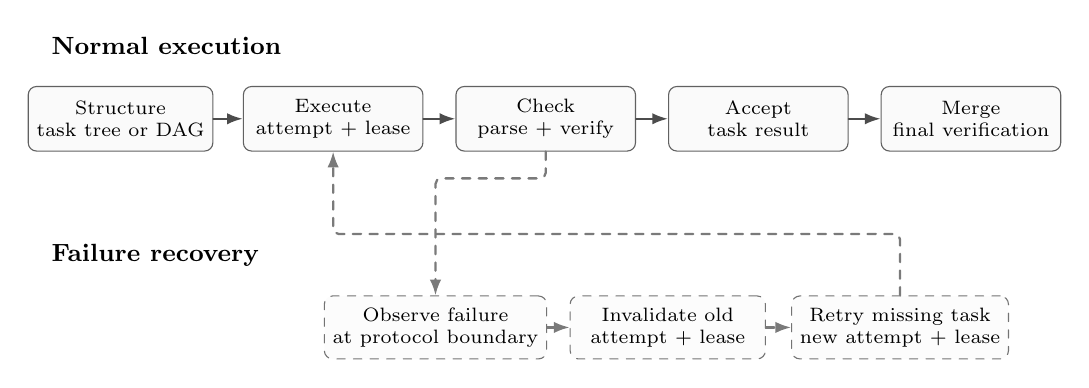
\begin{tikzpicture}[
  line cap=round,
  line join=round,
  stage/.style={
    draw=black!62,
    rounded corners=3pt,
    fill=black!2,
    minimum width=2.28cm,
    minimum height=0.82cm,
    align=center,
    font=\scriptsize,
    inner sep=3pt
  },
  recovery/.style={
    draw=black!55,
    rounded corners=3pt,
    dashed,
    fill=black!1,
    minimum width=2.48cm,
    minimum height=0.80cm,
    align=center,
    font=\scriptsize,
    inner sep=3pt
  },
  arrow/.style={
    -{Latex[length=2mm,width=1.45mm]},
    line width=0.82pt,
    draw=black!70
  },
  return/.style={
    -{Latex[length=2mm,width=1.45mm]},
    line width=0.82pt,
    dashed,
    draw=black!52
  }
]

% ------------------------------------------------
% Normal execution
% ------------------------------------------------
\node[font=\bfseries\small, anchor=west] at (-0.15,1.58)
{Normal execution};

\node[stage] (graph) at (0.85,0.65)
{Structure\\task tree or DAG};

\node[stage] (run) at (3.55,0.65)
{Execute\\attempt + lease};

\node[stage] (check) at (6.25,0.65)
{Check\\parse + verify};

\node[stage] (accept) at (8.95,0.65)
{Accept\\task result};

\node[stage] (merge) at (11.65,0.65)
{Merge\\final verification};

\draw[arrow] (graph) -- (run);
\draw[arrow] (run) -- (check);
\draw[arrow] (check) -- (accept);
\draw[arrow] (accept) -- (merge);

% ------------------------------------------------
% Failure recovery
% ------------------------------------------------
\node[font=\bfseries\small, anchor=west] at (-0.15,-1.08)
{Failure recovery};

\node[recovery] (observe) at (4.85,-2.00)
{Observe failure\\at protocol boundary};

\node[recovery] (invalidate) at (7.80,-2.00)
{Invalidate old\\attempt + lease};

\node[recovery] (retry) at (10.75,-2.00)
{Retry missing task\\new attempt + lease};

% Only one failure branch enters the recovery path.
\draw[return,rounded corners=2pt]
  (check.south)
  -- ++(0,-0.34)
  -| (observe.north);

% Recovery sequence.
\draw[return] (observe) -- (invalidate);
\draw[return] (invalidate) -- (retry);

% Return above the recovery boxes and enter the bottom of Execute.
% The crossing with the failure line is intentional and has no junction.
\draw[return,rounded corners=2pt]
  (retry.north)
  -- ++(0,0.78)
  -| (run.south);

\end{tikzpicture}%
}
\caption{
Normal execution structures a task, executes and checks its subtasks,
accepts verified task results, and performs the final merge and
verification. When a failure is observed, the protocol invalidates the
old attempt and lease, retries only the missing task with a new attempt
and lease, and returns it to the same execution path.
}
\label{fig:protocol-and-recovery-overview}
\end{figure}

In Normal execution, each execution of a task unit is recorded as an \emph{attempt}. The attempt is associated with a time-limited \emph{lease}, which specifies how long that execution remains valid. The executor---for example, a language model, external tool, or local program---returns a raw output. The task plugin first parses this output into the expected format and then verifies whether it satisfies the task-specific requirements. If the output passes these checks and the attempt is still valid, the protocol accepts it as the result of that task unit.

Only accepted results can be used by dependent task units or included in a merge. Once the required task-unit results are available, the plugin combines them according to the task-specific merge rule and performs a final verification of the root result. This separates output generation from result acceptance: an executor proposes a result, while the protocol and task-specific checks determine whether that result can affect the rest of the task.

Failure recovery follows the same execution flow. If an attempt fails, its lease expires, or its output does not pass the required checks, that attempt cannot provide an accepted result. When retry is allowed, the protocol creates a new attempt with a new lease for the same missing task unit. The replacement execution must pass the same parsing, verification, and result-acceptance steps as the original one. Results that were already accepted from other task units are preserved, so the protocol retries only the work that is still missing.

TokenMosaic separates domain-independent coordination from task-specific logic. The protocol coordinator manages task assignment, execution attempts, leases, retries, and the use of accepted results, while a task-specific module defines how the task is decomposed, how outputs are verified, and how accepted results are combined. Executors only perform assigned work and return outputs. This separation allows the same protocol flow to support different task domains without embedding domain-specific reasoning in the coordinator.

\subsection{Coordinating through Task Graphs}
\label{subsec:task-graph-coordination}

TokenMosaic coordinates complex tasks through explicit task graphs. Rather than prescribing a universal method for decomposing a task, it separates task-specific decomposition from protocol execution. A task-specific module provides the task graph, while the protocol coordinator manages how the tasks in that graph are scheduled and advanced. In this sense, the task graph connects task-specific problem solving to a common protocol flow: once the required task structure is provided, the coordinator does not need to encode the domain-specific reasoning that produced it.

For a task graph to enter this flow, it must specify the subtasks to be executed, their inputs and expected outputs, the dependencies among them, and the rules for verifying and merging their results. These dependencies determine which subtasks can currently run. A subtask whose required inputs are available is marked \textsc{Ready}, whereas a subtask that still depends on unresolved predecessors remains \textsc{Blocked}. During execution, only verified and accepted predecessor results can satisfy these dependencies. Once all required predecessor results have been accepted, the dependent subtask becomes ready for scheduling.

Figure~\ref{fig:task-graph-examples-balanced} shows how two different task structures are handled by the same protocol flow. In Factorization, the task-specific module divides the candidate divisor space into independent ranges. For example, factoring $221$ requires searching only
\[
[2,\lfloor\sqrt{221}\rfloor]=[2,14],
\]
which can be divided into $[2,5]$, $[6,9]$, and $[10,14]$. These range tasks have no dependencies on one another and can therefore be scheduled in parallel. Lean theorem proving uses a different structure. If lemma $L_3$ depends on $L_1$ and $L_2$, then $L_1$, $L_2$, and an independent lemma $L_4$ may be scheduled concurrently, while $L_3$ remains blocked until the results of both predecessors have been checked and accepted. The graph structure is task specific, but the same readiness and scheduling rules apply to both.

The current implementation uses deterministic task graphs supplied by the task-specific modules: Factorization uses predefined range partitions, while Lean uses preregistered proof plans or lemma DAGs. Executors generate candidate outputs for assigned subtasks but do not discover or modify the task graph. More generally, the protocol does not require every task family to use the same decomposition procedure; what it requires is an explicit task graph together with task-specific verification and merge rules. Once such a graph has been instantiated, TokenMosaic can apply the same execution flow to its ready subtasks. We next describe how these subtasks are assigned, executed, verified, and accepted.

\begin{figure}[!h]
\centering
\resizebox{0.97\linewidth}{!}{%
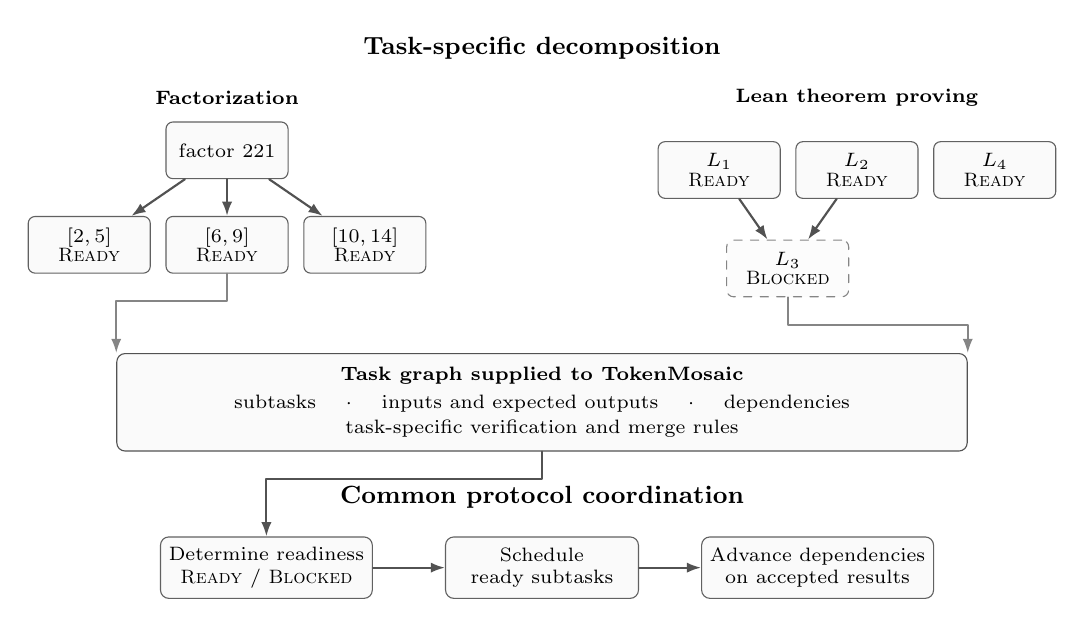
\begin{tikzpicture}[
  line cap=round,
  line join=round,
  task/.style={
    draw=black!62,
    rounded corners=2.5pt,
    fill=black!2,
    minimum width=1.55cm,
    minimum height=0.72cm,
    align=center,
    font=\scriptsize,
    inner sep=3pt
  },
  blocked/.style={
    draw=black!48,
    rounded corners=2.5pt,
    dashed,
    fill=black!1,
    minimum width=1.55cm,
    minimum height=0.72cm,
    align=center,
    font=\scriptsize,
    inner sep=3pt
  },
  spec/.style={
    draw=black!68,
    rounded corners=3pt,
    fill=black!2,
    minimum width=10.8cm,
    minimum height=1.05cm,
    align=center,
    font=\scriptsize,
    inner sep=5pt
  },
  protocol/.style={
    draw=black!62,
    rounded corners=3pt,
    fill=black!2,
    minimum width=2.45cm,
    minimum height=0.78cm,
    align=center,
    font=\scriptsize,
    inner sep=3pt
  },
  arrow/.style={
    -{Latex[length=1.8mm,width=1.3mm]},
    line width=0.78pt,
    draw=black!68
  },
  softarrow/.style={
    -{Latex[length=1.8mm,width=1.3mm]},
    line width=0.72pt,
    draw=black!48
  }
]

% =========================================================
% Upper level: task-specific structures
% =========================================================

\node[font=\bfseries\small] at (0,3.35)
{Task-specific decomposition};

% ---------------- Factorization ----------------

\node[font=\bfseries\scriptsize] at (-4.0,2.72)
{Factorization};

\node[task] (froot) at (-4.0,2.05)
{factor $221$};

\node[task] (fr1) at (-5.75,0.85)
{$[2,5]$\\[-1pt]\textsc{Ready}};

\node[task] (fr2) at (-4.0,0.85)
{$[6,9]$\\[-1pt]\textsc{Ready}};

\node[task] (fr3) at (-2.25,0.85)
{$[10,14]$\\[-1pt]\textsc{Ready}};

\draw[arrow] (froot) -- (fr1);
\draw[arrow] (froot) -- (fr2);
\draw[arrow] (froot) -- (fr3);


% ---------------- Lean ----------------

\node[font=\bfseries\scriptsize] at (4.0,2.72)
{Lean theorem proving};

\node[task] (l1) at (2.25,1.80)
{$L_1$\\[-1pt]\textsc{Ready}};

\node[task] (l2) at (4.0,1.80)
{$L_2$\\[-1pt]\textsc{Ready}};

\node[task] (l4) at (5.75,1.80)
{$L_4$\\[-1pt]\textsc{Ready}};

\node[blocked] (l3) at (3.12,0.55)
{$L_3$\\[-1pt]\textsc{Blocked}};

\draw[arrow] (l1) -- (l3);
\draw[arrow] (l2) -- (l3);


% =========================================================
% Shared representation
% =========================================================

\node[spec] (spec) at (0,-1.15) {
\textbf{Task graph supplied to TokenMosaic}\\[2pt]
subtasks \quad $\cdot$ \quad inputs and expected outputs
\quad $\cdot$ \quad dependencies\\[1pt]
task-specific verification and merge rules
};

% From the two task structures to the common representation
\draw[softarrow] (fr2.south) -- ++(0,-0.35) -| (spec.north west);
\draw[softarrow] (l3.south) -- ++(0,-0.35) -| (spec.north east);


% =========================================================
% Lower level: common protocol coordination
% =========================================================

\node[font=\bfseries\small] at (0,-2.35)
{Common protocol coordination};

\node[protocol] (ready) at (-3.5,-3.25)
{Determine readiness\\\textsc{Ready} / \textsc{Blocked}};

\node[protocol] (schedule) at (0,-3.25)
{Schedule\\ready subtasks};

\node[protocol] (advance) at (3.5,-3.25)
{Advance dependencies\\on accepted results};

\draw[arrow] (spec.south) -- ++(0,-0.35) -| (ready.north);
\draw[arrow] (ready) -- (schedule);
\draw[arrow] (schedule) -- (advance);

\end{tikzpicture}%
}

\caption{
Different task-specific modules expose different task-graph structures to the same TokenMosaic protocol. Factorization produces independent range tasks that can be scheduled in parallel, whereas Lean may contain dependency-constrained tasks that remain blocked until their predecessors are accepted. Once the task graph and its task-specific verification and merge rules are provided, the protocol coordinator applies the same readiness and scheduling process without encoding the domain-specific decomposition logic.
}
\label{fig:task-graph-examples-balanced}
\end{figure}

\subsection{Executing and Verifying Task Units}
\label{subsec:verified-execution}

Once a task unit is \textsc{Ready}, the scheduler selects a compatible worker according to its required capabilities. Scheduling creates a new attempt and a corresponding lease. The execution request binds the root task, unit, input artifacts, expected output contract, worker, attempt, lease, deadline, and fencing identity. This binding answers a basic question that ordinary multi-agent conversations often leave implicit: which execution is currently allowed to speak for this unit?

A submission is admitted only if it still belongs to the active attempt and lease. The task, unit, attempt, lease, and fencing identity must match the latest ledger state, and the result must arrive before the lease expires. A late or mismatched output may still be stored as evidence of what the worker produced, but it cannot advance the task. Physical arrival and protocol authority are therefore separate facts.

An admitted output then passes through the evidence gates in Figure~\ref{fig:evidence-gates-balanced}. The plugin parses provider-specific text into the declared schema, the protocol checks artifact integrity and required output coverage, and the plugin applies the domain-specific verifier. Only a candidate that passes all required checks is eligible for canonical selection. Under the current policy, the earliest fully verified bundle in ledger order becomes the unique canonical output of the task unit; other verified candidates remain available for audit.

\begin{figure}[!h]
\centering
\resizebox{0.94\linewidth}{!}{%
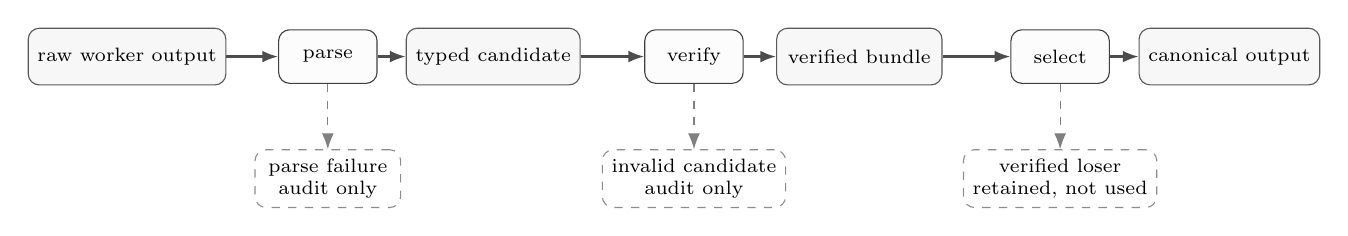
\begin{tikzpicture}[
  object/.style={
    draw=black!65,
    rounded corners,
    fill=black!3,
    minimum width=2.1cm,
    minimum height=0.72cm,
    align=center,
    font=\scriptsize
  },
  gate/.style={
    draw=black!75,
    rounded corners,
    fill=black!1,
    minimum width=1.25cm,
    minimum height=0.68cm,
    align=center,
    font=\scriptsize
  },
  audit/.style={
    draw=black!45,
    rounded corners,
    dashed,
    minimum width=1.85cm,
    minimum height=0.62cm,
    align=center,
    font=\scriptsize
  },
  arrow/.style={-{Latex[length=2mm]}, thick, draw=black!70},
  reject/.style={-{Latex[length=2mm]}, dashed, draw=black!50}
]
  \node[object] (raw) at (0,0.55) {raw worker output};
  \node[gate] (parse) at (2.55,0.55) {parse};
  \node[object] (typed) at (4.65,0.55) {typed candidate};
  \node[gate] (verify) at (7.2,0.55) {verify};
  \node[object] (valid) at (9.3,0.55) {verified bundle};
  \node[gate] (select) at (11.85,0.55) {select};
  \node[object] (canon) at (14.0,0.55) {canonical output};

  \draw[arrow] (raw) -- (parse);
  \draw[arrow] (parse) -- (typed);
  \draw[arrow] (typed) -- (verify);
  \draw[arrow] (verify) -- (valid);
  \draw[arrow] (valid) -- (select);
  \draw[arrow] (select) -- (canon);

  \node[audit] (pbad) at (2.55,-1.0) {parse failure\\audit only};
  \node[audit] (vbad) at (7.2,-1.0) {invalid candidate\\audit only};
  \node[audit] (loser) at (11.85,-1.0) {verified loser\\retained, not used};
  \draw[reject] (parse) -- (pbad);
  \draw[reject] (verify) -- (vbad);
  \draw[reject] (select) -- (loser);
\end{tikzpicture}%
}
\caption{Generation is not authority. Many outputs may be stored, but only a current, parsed, verified, and selected bundle becomes the canonical output consumed by later units.}
\label{fig:evidence-gates-balanced}
\end{figure}

The following implementation sketch makes the same boundary concrete. It is intentionally abstract: the full implementation also persists artifacts, verification reports, and ledger events. The essential point is that current execution authority is checked before parsing, and canonical binding is considered only after the plugin has produced an eligible verification report.

\begin{figure}[!h]
\centering
\begin{minipage}{0.94\linewidth}
\small
\begin{verbatim}
def process_submission(submission, attempt, lease, plugin):
    if not matches_current_authority(submission, attempt, lease):
        record_audit_only(submission)
        return

    candidate = plugin.parse(submission.raw_output)
    report = plugin.verify(candidate)
    record_verification(report)

    if report.eligible_for_canonical:
        bind_first_verified(submission.unit_id)
\end{verbatim}
\end{minipage}
\caption{Abstracted normal-path code. The executor supplies a candidate, while the current lease, plugin verifier, and canonical-selection rule determine whether the candidate can influence the shared task.}
\label{fig:submission-code-balanced}
\end{figure}

For factorization, the verifier checks that a claimed factor lies in the assigned range and divides the target. If the worker responsible for $[10,14]$ returns $13$, the result becomes useful only after confirming
\begin{equation}
13\in[10,14]
\qquad\text{and}\qquad
221\bmod 13=0.
\label{eq:factor-example}
\end{equation}
For a no-factor result, the verifier also checks the range identity and later requires complete coverage before a negative conclusion is accepted. For Lean, TokenMosaic reconstructs the proof in the fixed Lean/Lake environment and invokes the real checker. Plausible proof text is therefore kept outside canonical state unless the checker accepts it for the registered theorem payload.

\subsection{Composing the Final Result}
\label{subsec:result-composition}

A decomposition is useful only if the accepted child results can be recomposed into a valid parent result. Every decomposition proposal therefore includes a versioned merge plan. The plan identifies the expected parent outputs, the child output slots from which they are derived, and the evidence-sufficiency rule that decides whether the merge should \textsf{wait}, become \textsf{ready}, or become \textsf{failed}.

Evidence sufficiency is domain dependent. Table~\ref{tab:merge-sufficiency-balanced} compares the three cases that are most important for understanding the implementation. The table also explains why merge cannot be reduced to concatenating strings or waiting for all worker processes to stop: the required evidence and final check depend on the claim being made.

\begin{table}[!h]
\centering
\small
\renewcommand{\arraystretch}{1.16}
\caption{Different meanings of sufficient child evidence under one merge lifecycle.}
\label{tab:merge-sufficiency-balanced}
\begin{tabularx}{\linewidth}{@{}p{0.20\linewidth}>{\raggedright\arraybackslash}X>{\raggedright\arraybackslash}X@{}}
\toprule
\textbf{Parent claim} & \textbf{Merge is ready when} & \textbf{Independent final check} \\
\midrule
Factorization: a factor exists & At least one canonical range result contains a verified non-trivial factor witness & Recheck the factor and arithmetic recomposition \\
Factorization: no factor exists & Canonical no-factor evidence covers every required range without gaps or overlap & Recheck complete coverage of $[2,\lfloor\sqrt{n}\rfloor]$ \\
Lean root theorem & Every required lemma slot has a checker-accepted canonical proof with the correct dependency binding & Assemble the root proof and invoke Lean again on the root theorem \\
\bottomrule
\end{tabularx}
\end{table}

When the merge is ready, TokenMosaic creates an explicit merge task whose inputs are the selected canonical child artifacts. The merge task follows the same lifecycle as every other unit: it receives an execution request, produces an output, passes task-specific verification, and obtains a canonical result. A successful child merge may resolve a parent output, activate another dependent unit, or satisfy a higher-level merge plan. The root task is complete only when every required root output has been resolved and the root-specific verification succeeds.

This design yields a continuous evidence chain. Local worker outputs become canonical unit results; canonical unit results justify merge inputs; verified merge outputs resolve parent slots; and the root result remains connected to every child artifact, checker report, and execution authority on which it depends.

\subsection{Persistent Evidence and Replay}
\label{subsec:persistent-evidence}

TokenMosaic stores two complementary kinds of history. Artifacts answer \emph{what was produced}: root inputs, execution requests, raw responses, parsed candidates, checker reports, decomposition plans, merge inputs, and final outputs. Ledger events answer \emph{why it counted}: which attempt was active, whether a submission was admitted, which verification passed, which output became canonical, and how a parent was completed. An artifact may exist without influencing the task; it acquires protocol meaning only when an authoritative event binds it to a state transition.

The event ledger is append-only and hash-linked, while the SQLite index is a rebuildable query view rather than a second source of truth. Replay reconstructs task state from the persisted events and artifacts instead of invoking the executor again. A root result can therefore be traced backward through its merge record, selected child outputs, verification reports, submissions, attempts, leases, execution requests, and original inputs.

This distinction also clarifies the meaning of contribution in TokenMosaic. Spending model tokens, compute, checker time, or human effort creates an execution artifact. It becomes accepted contribution evidence only after it passes the declared parser and verifier, becomes canonical, and supports a completed dependency or merge. The protocol therefore accounts for useful accepted work rather than raw expenditure alone.


\section{Fault Tolerance and Recovery}
\label{sec:bounded-recovery}

Section~\ref{sec:tokenmosaic-protocol} describes the normal path. In practice, a worker may disappear, a provider may return an error, a response may fail to parse, a verifier may reject the candidate, or an otherwise useful output may arrive after its lease has expired. TokenMosaic handles these cases without creating a separate shortcut around verification. Recovery closes the old authority, creates a fresh attempt when policy allows it, and sends the replacement through the same evidence gates shown in Figure~\ref{fig:evidence-gates-balanced}.

\subsection{Failure Model and Safety Principle}
\label{subsec:failure-model}

A runtime anomaly becomes a protocol failure when it reaches a boundary at which normal progress can no longer continue. Table~\ref{tab:failure-boundaries-balanced} maps each boundary to the fact observed by the protocol and the resulting interpretation. The common retry rule operates over these typed observations, while the parent merge policy separately decides whether the missing unit is still necessary.

\begin{table}[!h]
\centering
\scriptsize
\renewcommand{\arraystretch}{1.16}
\caption{Boundary-aligned failure observations.}
\label{tab:failure-boundaries-balanced}
\begin{tabularx}{\linewidth}{@{}p{0.16\linewidth}p{0.25\linewidth}p{0.20\linewidth}X@{}}
\toprule
\textbf{Boundary} & \textbf{Observable fact} & \textbf{Old attempt} & \textbf{Protocol meaning} \\
\midrule
Worker / transport & Explicit executor error & \textsc{Failed} & No usable submission was produced; evaluate the replacement budget \\
Lease / liveness & Lease expires or no result arrives in time & \textsc{Superseded} & The execution authority has ended; later output is stale \\
Parser & Admitted raw output cannot satisfy the output schema & \textsc{Rejected} & No typed candidate exists for verification \\
Verifier or checker & Candidate fails arithmetic, artifact, evidence, audit, or Lean checks & \textsc{Rejected} & Candidate cannot become canonical \\
Composition & Required canonical child evidence is absent or terminally impossible & Child facts unchanged & Merge remains \textsf{wait} or becomes \textsf{failed} according to evidence sufficiency \\
\bottomrule
\end{tabularx}
\end{table}

Although these failures occur at different stages, they are governed by one safety condition. For any artifact $x$ that influences a dependency, merge, parent output, or root result, TokenMosaic requires
\begin{equation}
\operatorname{Influence}(x)
\Rightarrow
\operatorname{Current}(x)
\land
\operatorname{Parsed}(x)
\land
\operatorname{Verified}(x)
\land
\operatorname{Canonical}(x).
\label{eq:failure-safety-balanced}
\end{equation}
A failed or stale output may still be persisted for audit, cost analysis, and debugging, but persistence alone does not grant authority. The same principle applies to control operations: scheduling, recovery, verification, and merge decisions are evaluated against the latest ledger-derived state, and conflicting reuse of an accepted operation identity is rejected.

\subsection{Containing Failure and Reassigning Work}
\label{subsec:containment-reassignment}

Recovery begins by closing the authority associated with the failed execution. An expired lease becomes terminal and its unfinished attempt is superseded; an executor error fails the attempt; and parser, verifier, or checker rejection closes the candidate path as rejected. The protocol records the old terminal state together with the next state of the task unit. A unit cannot be reopened for a replacement while its previous lease remains active.

The replacement decision is bounded. Let $K$ be the maximum number of replacement attempts allowed after the initial execution. Then
\begin{equation}
N_{\mathrm{attempts}}(u)\leq 1+K.
\label{eq:retry-limit-balanced}
\end{equation}
If another replacement is permitted, the unit returns to \textsc{Ready}; otherwise it enters \textsc{Failed}. Returning to \textsc{Ready} authorizes another scheduling decision, but it does not mean that the unit has recovered.

The code-level decision is correspondingly small. It closes the current execution path and decides only whether the unit may be scheduled again. A later scheduler call creates fresh authority, and the replacement is counted as recovered only after it establishes a new canonical output.

\begin{figure}[!h]
\centering
\begin{minipage}{0.94\linewidth}
\small
\begin{verbatim}
def recovery_decision(trigger, retry_count, max_retries):
    close_current_authority(trigger)

    # max_retries counts replacements after the initial attempt.
    retry_allowed = retry_count <= max_retries
    next_unit_state = READY if retry_allowed else FAILED
    return next_unit_state

# READY authorizes scheduling; it does not yet mean RECOVERED.
\end{verbatim}
\end{minipage}
\caption{Abstracted bounded-recovery code. Retry authorization, creation of a fresh attempt, and successful recovery are deliberately separate protocol facts.}
\label{fig:recovery-code-balanced}
\end{figure}

Figure~\ref{fig:recovery-state-balanced} shows the resulting authority transition. A replacement receives a fresh attempt, lease, deadline, and fencing identity. It reads the same persisted inputs and canonical predecessor outputs, but it does not inherit hidden state from the failed worker. A late output from the old attempt remains visible in the audit history while failing the current-authority check before verification.

\begin{figure}[!h]
\centering
\resizebox{0.96\linewidth}{!}{%
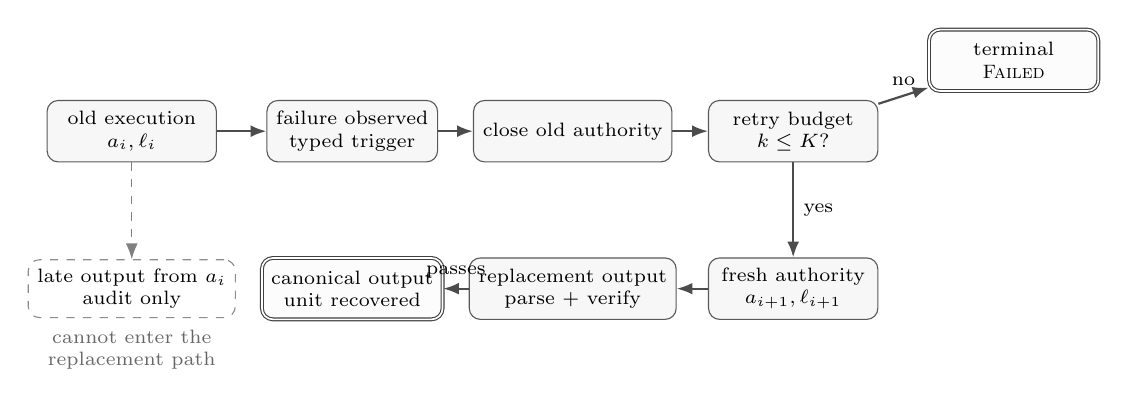
\begin{tikzpicture}[
  state/.style={
    draw=black!65,
    rounded corners,
    fill=black!3,
    minimum width=2.15cm,
    minimum height=0.78cm,
    align=center,
    font=\scriptsize
  },
  terminal/.style={
    draw=black!75,
    rounded corners,
    double,
    fill=black!1,
    minimum width=2.15cm,
    minimum height=0.78cm,
    align=center,
    font=\scriptsize
  },
  audit/.style={
    draw=black!45,
    rounded corners,
    dashed,
    minimum width=2.05cm,
    minimum height=0.65cm,
    align=center,
    font=\scriptsize
  },
  arrow/.style={-{Latex[length=2mm]}, thick, draw=black!70},
  stale/.style={-{Latex[length=2mm]}, dashed, draw=black!50}
]
  \node[state] (old) at (0,1.15) {old execution\\$a_i,\ell_i$};
  \node[state] (fault) at (2.8,1.15) {failure observed\\typed trigger};
  \node[state] (closed) at (5.6,1.15) {close old authority};
  \node[state] (decision) at (8.4,1.15) {retry budget\\$k\leq K$?};
  \node[terminal] (failed) at (11.2,2.05) {terminal\\\textsc{Failed}};

  \draw[arrow] (old) -- (fault);
  \draw[arrow] (fault) -- (closed);
  \draw[arrow] (closed) -- (decision);
  \draw[arrow] (decision) -- node[above,font=\scriptsize]{no} (failed);

  \node[state] (fresh) at (8.4,-0.85) {fresh authority\\$a_{i+1},\ell_{i+1}$};
  \node[state] (candidate) at (5.6,-0.85) {replacement output\\parse + verify};
  \node[terminal] (recovered) at (2.8,-0.85) {canonical output\\unit recovered};
  \draw[arrow] (decision) -- node[right,font=\scriptsize]{yes} (fresh);
  \draw[arrow] (fresh) -- (candidate);
  \draw[arrow] (candidate) -- node[above,font=\scriptsize]{passes} (recovered);

  \node[audit] (late) at (0,-0.85) {late output from $a_i$\\audit only};
  \node[font=\scriptsize,align=center,text=black!60] at (0,-1.62)
  {cannot enter the\\replacement path};
  \draw[stale] (old) -- (late);
\end{tikzpicture}%
}
\caption{Recovery replaces execution authority rather than extending it. The old attempt is closed before a fresh attempt is scheduled. A late output remains auditable but cannot enter the replacement's verification path.}
\label{fig:recovery-state-balanced}
\end{figure}

Consider the range $[10,14]$ in the factorization of $221$. Worker $w_0$ receives the range under $(a_0,\ell_0)$ but stops sending heartbeats. After $\ell_0$ expires, the protocol supersedes $a_0$ and returns the unit to \textsc{Ready}. Worker $w_1$ receives the same persisted range under fresh $(a_1,\ell_1)$. A late answer $13$ from $a_0$ is stored but rejected as stale. The answer $13$ from $a_1$ is parsed, verified by Equation~\ref{eq:factor-example}, and canonically bound. Only this last event establishes recovery.

The example separates three facts that are often conflated. \emph{Retry authorized} means policy permits another attempt. \emph{Replacement created} means the scheduler issued fresh authority. \emph{Recovered} means the replacement completed admission, parsing, verification, and canonicalization. A replacement may fail again, in which case the same bounded rule is applied until a canonical output is established or the retry budget is exhausted.

\subsection{Resuming from Verified Progress}
\label{subsec:graph-level-recovery}

TokenMosaic retries the missing task unit rather than restarting the root task. Canonical outputs from unaffected units remain immutable and reusable. The graph waits only at the point where accepted evidence is missing. When a replacement produces the required canonical output, blocked successors become ready and normal execution resumes.

The parent merge policy is re-evaluated whenever a child becomes canonical or reaches terminal failure. Table~\ref{tab:graph-recovery-balanced} shows why the effect of one failed worker depends on the parent claim rather than on process failure alone.

\begin{table}[!h]
\centering
\small
\renewcommand{\arraystretch}{1.16}
\caption{Graph-aware recovery preserves accepted work and regenerates only missing evidence.}
\label{tab:graph-recovery-balanced}
\begin{tabularx}{\linewidth}{@{}p{0.24\linewidth}X X@{}}
\toprule
\textbf{Scenario} & \textbf{What is preserved} & \textbf{When the root can continue} \\
\midrule
Factorization: another range has a valid factor & The canonical factor witness and all completed range evidence & Immediately after the witness is sufficient for a positive merge; the failed range may no longer be needed \\
Factorization: the target may be prime & All completed no-factor range certificates & Only after the missing range is recovered and the complete candidate domain is canonically covered \\
Lean: $L_2$ fails while $L_1$ is accepted & Canonical proof of $L_1$ and unrelated accepted lemmas & After a replacement proof of $L_2$, then its dependent nodes, and finally a successful root check \\
Lean: a required lemma exhausts retries & All other accepted proof artifacts & The root cannot complete if the registered merge rule still requires the failed lemma \\
\bottomrule
\end{tabularx}
\end{table}

This graph-level behavior avoids two opposite errors. Restarting the entire task would waste verified work, while ignoring the missing evidence could permit an incomplete root result. TokenMosaic instead preserves accepted branches, regenerates only the missing contribution, and lets the registered evidence-sufficiency rule decide whether that contribution is still necessary.

\subsection{Recovery Outcomes and Guarantees}
\label{subsec:recovery-outcomes}

A recovery episode has three possible outcomes. In the common case, a replacement establishes a canonical output, activates dependent units, and returns the task to normal execution. In some tasks, the missing unit becomes unnecessary because other canonical evidence already satisfies the merge rule; a verified factor witness is the main example. In the terminal case, the retry budget is exhausted while the result remains required, so the unit enters \textsc{Failed} and the corresponding parent path remains unresolved or becomes failed.

TokenMosaic does not guarantee that every task will eventually succeed. A model may repeatedly produce invalid candidates, a provider or checker may remain unavailable, or a task may require evidence that cannot be obtained within the configured budget. The protocol offers a narrower guarantee: old authority is closed before replacement, stale and invalid outputs remain outside canonical state, retries are finite, accepted progress is preserved, and every parent outcome follows an explicit evidence-sufficiency rule.

Together, Sections~\ref{sec:tokenmosaic-protocol} and~\ref{sec:bounded-recovery} describe one design. Normal execution converts candidate work into a verified root result; recovery replaces failed authority and returns only the missing unit to the same evidence path. In both cases, progress is defined by newly established canonical evidence rather than raw execution or token expenditure.









\section{Experimental Tasks and Evaluation Design}
\label{sec:experimental-design}

TokenMosaic is evaluated through two complementary task suites and five
controlled experiments. The workloads expose different task-graph
structures, verification procedures, and execution constraints, allowing
the system's design properties to be examined through observable protocol
behavior.

The evaluation distinguishes protocol completion from valid task
completion. A root task counts as a valid completion only when it reaches
the completed state and its accepted output passes the authoritative
task-specific verifier or checker. This distinction separates the
protocol's ability to advance a task from its ability to produce a correct
end-to-end result.


\subsection{Experimental Task Suites}

The evaluation uses Integer Factorization and Lean theorem proving because
they represent complementary forms of decomposable work. Factorization
provides broad parallel search over independent candidate ranges and an
inexpensive deterministic verifier. Lean provides dependency-constrained
proof construction and a deterministic checker operating in a fixed
formal environment.

The two task suites share the same protocol objects and execution
lifecycle, but instantiate different input contracts, task graphs,
parsers, validity procedures, and merge rules. They therefore provide a
controlled basis for examining whether one coordination protocol can
operate across different domain-specific plugin contracts.


\subsubsection{Integer Factorization Tasks}

The Factorization corpus used by Experiment~1 contains 300 root tasks,
with 100 easy, 100 medium, and 100 hard cases. Each task supplies an integer \(n\) and
requires either a non-trivial factor or a verified no-factor conclusion
over the complete candidate domain
\[
[2,\lfloor\sqrt{n}\rfloor].
\]

A positive candidate \(d\) is valid when
\[
1<d<n
\qquad\text{and}\qquad
n\bmod d=0.
\]
A no-factor result requires accepted and canonical coverage of every
required candidate range. The catalog includes semiprimes whose factors
occur at early, middle, and late positions in the candidate domain,
together with seven hard prime controls that require complete range
coverage.

Difficulty changes the task-graph granularity while preserving the
complete candidate domain. The standard easy, medium, and hard profiles
produce 2, 4, and 8 contiguous range units, respectively. The
Factorization plugin generates the range boundaries, verifies complete
coverage, and binds the units to declared merge slots. AI workers search
only their assigned ranges. Their outputs pass through the task parser
and deterministic verifier before they can contribute to the canonical
root result.

The deterministic plan for each selected case is frozen before execution.
In particular, the worker-scaling experiment reuses the complete plan of
the corresponding Experiment~1 case---including its ranges, identifiers,
prompts, and dependencies---rather than substituting an experiment-specific
split profile.

The Factorization suite makes three forms of evidence directly observable.
Its certified range partitions expose whether a plugin plan is converted
into the intended task graph. Its independent units expose how worker
capacity affects parallel execution. Its inexpensive verifier exposes
whether generated candidates are checked before they affect the canonical
root result.


\subsubsection{Lean Theorem-Proving Tasks}

The Lean catalog contains 135 root theorems organized as a
\(3\times3\) matrix. The three paper difficulty levels are
\texttt{simple}, \texttt{medium\_lemma\_dag}, and
\texttt{hard\_frontier}. The three topic families are
\texttt{pure\_logic}, \texttt{function\_set}, and
\texttt{induction}. Each difficulty--topic cell contains exactly
15 theorems.

Simple tasks use shallow proof structures and short dependency chains.
Medium tasks use preregistered lemma dependency graphs with two or three
levels. Hard-frontier tasks use deeper dependency structures and combine
operations such as induction, rewriting, auxiliary lemmas, and theorem
reuse. Every paper-eligible theorem is accompanied by a fixed environment
identity, a versioned proof plan, and a checker-backed oracle package that
passes catalog preflight.

For a theorem statement \(s\), proof candidate \(y\), and fixed Lean
environment \(\Omega\), validity is defined by
\[
V_{\mathrm{Lean}}(s,y,\Omega)=
\begin{cases}
1, & \text{if the assembled proof is accepted in } \Omega,\\
0, & \text{otherwise}.
\end{cases}
\]

The executable lemma graph is obtained from a versioned preregistered plan
and validated by the Lean plugin. AI workers generate proof candidates for
the assigned lemma or proof units. Each candidate is checked in the fixed
local Lean, Lake, toolchain, and library environment. A root theorem counts
as valid only when the required child proofs satisfy their dependency and
slot bindings, the proof files are assembled according to the validated
plan, and the final root check succeeds.

The Lean suite exposes dependency-sensitive decomposition and composition.
Its versioned lemma graphs make the expected units and dependency edges
explicit, while per-unit checking and final root checking distinguish
locally valid proof artifacts from a valid assembled theorem.


\subsection{Controlled Execution Conditions}

Experiment~1 and Experiment~5 use real AI API execution. Every real AI
attempt records the request fact, raw model output, parsed candidate or
parse failure, provider and model identity, latency, token usage, cost
estimate, and the references connecting these records to the corresponding
protocol attempt. Experiment~1 uses the official DeepSeek
\texttt{deepseek-v4-flash} baseline with thinking enabled. Experiment~5
uses the three preregistered SiliconFlow endpoints described below.

Experiments~2--4 make no new provider calls. They replay the persisted
Experiment~1 per-unit traces after matching the case, source repeat, planned
unit, and ordinary domain semantics. Source usage and latency remain
trace-attributed facts; logical scheduling or deterministic perturbation is
identified explicitly as simulated. Catalog versions, task order, prompts,
parser and plugin versions, request limits, and execution policies remain
fixed within each comparison group except for the preregistered independent
variable.

The task graph remains part of the versioned task specification.
Factorization ranges are generated by deterministic plugin rules, while
Lean dependency graphs are obtained from preregistered plans validated by
the Lean plugin. AI execution is therefore measured as candidate production
within an explicit task graph. Plan identities, graph-construction
evidence, parser decisions, verification results, canonical bindings, and
merge evidence are persisted as parts of the same run record.


\subsection{Experimental Program}

\paragraph{Experiment 1: Cross-Domain Feasibility and Task Difficulty.}

Experiment 1 executes the two task suites under a shared protocol
configuration in order to compare their task-graph construction,
domain-specific validation, and end-to-end completion behavior. It uses
300 Factorization roots and all 135 Lean roots. Each root is executed
once with 10 workers using the official DeepSeek
\texttt{deepseek-v4-flash} baseline. This gives 435 preregistered roots.

Factorization tasks are grouped by easy, medium, and hard difficulty.
Lean tasks are grouped by the complete difficulty--topic matrix. For each
group, the experiment records root completion, accepted validity, parser
and verifier or checker status, split and child counts, merge status,
wall-clock time, provider latency, token usage, cost per completed task,
and failure stage.

For each domain or Lean topic family, the highest tested difficulty
containing at least one valid completion is recorded as the highest
observed valid-completion difficulty. This value is reported together with
the complete group-level completion and validity rates, so that an isolated
successful task does not replace the distribution over the task set.

The comparison uses the same root, task-unit, attempt, event, and artifact
contracts in both domains. The protocol core and execution lifecycle remain
fixed, while the plugin supplies the domain-specific task graph, parser,
verifier or checker, and merge procedure.


\paragraph{Experiment 2: Worker Scaling.}

Experiment 2 uses 50 hard Factorization cases. Every case inherits its
complete Experiment~1 plan, unit semantics, prompts, dependencies, and
persisted per-unit traces. The worker count is
\[
w\in\{1,3,7,10,30,50\}.
\]
Each worker level executes the same ordered task set twice, giving
\(50\times6\times2=600\) preregistered roots. The source repeat is fixed at
zero while the two Experiment~2 repeats are scheduling repeats. No condition
makes a new provider call: the logical scheduler uses the matched source
attempts and source latency while preserving dependencies and early stop.

Worker count controls concurrent execution within one root task. The
experiment therefore measures the parallelism exposed by the task graph
rather than concurrency across unrelated root inputs.

A verifier-accepted factor witness may satisfy the root merge condition
before every range has been scheduled. Requests already dispatched in the
active batch are allowed to finish, while later unscheduled ranges remain
unexecuted. Prime controls require accepted coverage of all 20 ranges.
The evaluation records planned, dispatched, completed, in-flight, and
unscheduled units so that logical latency is interpreted together with
trace-attributed token and cost consumption.

The 30-worker and 50-worker conditions exceed the maximum width of the
inherited hard-case range plans. They expose the saturation region in which additional
configured capacity cannot increase the parallelism supplied by the task
graph. Configured worker count is therefore reported together with
observed peak concurrency and worker utilization.


\paragraph{Experiment 3: Controlled Faults and Worker Loss.}

Experiment 3 replays persisted Experiment~1 traces and injects a controlled
fault into the targeted unit's first attempt. Each transformation links the
source answer, transformed submission, injection point, and affected
protocol attempt. Replacement attempts read the matching natural source
attempt (or the deterministic last-attempt fallback); neither the fault run
nor its replacement makes a new provider call.

The five rate-based fault types are
\texttt{false\_positive}, \texttt{false\_negative},
\texttt{no\_return}, \texttt{late\_submission}, and
\texttt{executor\_error}.

Factorization uses a 50-root source slice with easy, medium, and hard counts
of 17, 17, and 16, respectively, at fault rates
\[
1\%,5\%,10\%,25\%,50\%,100\%.
\]
Lean uses a fixed three-task slice containing one task from each topic
family at rates
\[
10\%,50\%,100\%.
\]
Each condition is repeated twice. Zero percent is not a standalone
condition or experimental root; overhead is computed against the paired
no-fault reference for the same case and repeat.

Worker loss is evaluated separately with 10 workers. One or three executor
processes are terminated at target progress levels of 25\%, 50\%, and
75\%. The coordinator remains active while the protocol records process
termination, lease expiry, reassignment, replacement attempts, recovered
slots, and final root validity. Each worker-loss condition is repeated
twice and compared with its paired no-fault reference. Process termination
is real, while the model answers remain trace-backed.

For both fault and reference executions, token usage and latency are
deterministically perturbed from the source trace under the frozen seed.
Time, token, and cost overheads are therefore reported as simulated,
trace-attributed quantities rather than as new API consumption or observed
provider wall-clock.

These conditions distinguish three outcomes: detection and isolation of an
invalid or stale output, successful recovery through a replacement attempt,
and terminal failure after recovery opportunities are exhausted. The
classification is derived from verification, canonical-state, lease,
attempt, and root-completion evidence.


\paragraph{Experiment 4: Protocol Ablation.}

Experiment 4 compares the complete \texttt{FULL} condition with four
single-mechanism removals:
\texttt{NO\_VERIFICATION}, \texttt{NO\_PARSER\_POLICY},
\texttt{NO\_REQUEUE}, and \texttt{NO\_MERGE\_GATE}.
It also executes all six pairwise removals, giving 11 modes in total. Each
mode changes only the specified lifecycle decisions while preserving the
task, source trace, prompt, retry limit, and remaining execution policy.

The Factorization portion uses 50 fixed roots and the Lean portion uses
15 fixed roots: five from each difficulty level, with a fixed
\(2/2/1\) allocation across the three topic families. Each mode is
repeated three times, giving \(11\times3\times65=2{,}145\) preregistered
roots. All modes consume the same matched Experiment~1 traces and make zero
provider calls.

Before mode expansion, each case--repeat pair receives one deterministic,
mode-blind challenge: an invalid parsed candidate, parser-required canonical
JSON, a recoverable no-return, or a required-child delay. The same challenge
plan is replayed across all 11 modes, and the injector cannot observe which
mechanisms are disabled. Mechanism removal occurs before the corresponding
parser, verifier or checker, replacement, or merge-gate decision; it is not
implemented by running the mechanism and overwriting its outcome afterward.

The two acceptance-related ablations isolate the effects of typed parsing
and task-specific verification. The requeue ablation isolates the effect
of replacement attempts after a failed or expired attempt. The merge-gate
ablation tests the effect of dependency and required-slot checks before
root assembly.

In addition to completion, accepted validity, wall-clock time, token
consumption, and cost, the experiment records incorrect canonical
acceptance, raw-only exposure and acceptance, tasks left without a
replacement attempt, and premature merge attempts. Each observation is
derived from task-, attempt-, canonical-, recovery-, and merge-level
evidence rather than from the name of the ablation condition.


\paragraph{Experiment 5: Model--Provider Endpoint Comparison.}

Experiment 5 compares three preregistered model--provider endpoints:
SiliconFlow \texttt{zai-org/GLM-5.2}, SiliconFlow
\texttt{Qwen/Qwen3-14B}, and SiliconFlow
\texttt{MiniMaxAI/MiniMax-M2.5}. All three use their frozen thinking
configuration.

The comparison uses 28 hard Factorization roots and nine hard Lean roots,
with three Lean roots from each topic family. Every endpoint executes the
same 37 roots only at \texttt{repeat\_id=0}, giving 111 preregistered roots.
Replacement is disabled and each AI unit permits at most one provider
attempt. Task order, prompts, plugin and parser versions, request limits,
and endpoint-specific thinking profiles are frozen before execution.

Completion and accepted validity are the primary cross-endpoint measures.
Latency, cost, provider errors, and rate limiting are reported together
with provider identity because these quantities reflect both model
behavior and endpoint infrastructure. The unit of comparison is therefore
the registered model--provider endpoint rather than model architecture
alone.

DeepSeek \texttt{deepseek-v4-flash} is not a fourth Experiment~5 endpoint.
It may appear only as a supplemental reference that reuses committed
Experiment~1 facts; that reference is excluded from the formal endpoint
comparison and from latency comparison.


\subsection{Relationship Between the Experiments and the Design Desiderata}

The task suites and experimental conditions provide an empirical
interpretation of the five design desiderata. Each desideratum is assigned
to the experiment that provides its most direct test. This primary mapping
keeps the evidential role of each experiment explicit while allowing one
experiment to address different properties through distinct observations.

\begin{table}[t]
\centering
\caption{Primary experimental test for each TokenMosaic design desideratum.}
\label{tab:desiderata-primary-tests}
\footnotesize
\setlength{\tabcolsep}{3.5pt}
\renewcommand{\arraystretch}{1.18}
\begin{tabularx}{\linewidth}{
    >{\raggedright\arraybackslash}p{0.145\linewidth}
    >{\raggedright\arraybackslash}p{0.14\linewidth}
    >{\raggedright\arraybackslash}X
    >{\raggedright\arraybackslash}X}
\toprule
\textbf{Desideratum} &
\textbf{Primary experiment} &
\textbf{Why the experiment tests the property} &
\textbf{Principal evidence} \\
\midrule

\textbf{Decomposability}
&
Experiment 1
&
The two domains instantiate different task-graph structures: independent
Factorization ranges and dependency-ordered Lean lemma units. Their
execution tests whether declared plugin plans become executable graphs
that can be recomposed into valid root outputs.
&
Agreement between the versioned plan and created units; split and child
counts; dependency and required-slot bindings; merge status; final root
validity.
\\

\textbf{Local verifiability}
&
Experiment 4
&
The complete protocol is compared with all single and pairwise removals of
typed parsing, task-specific verification, requeue, and the merge gate.
Mode-blind challenges exercise the corresponding structural boundary under
matched cases and source traces.
&
Challenge injection and route evidence; accepted-validity rate; raw-only or
invalid acceptance; missing replacement; premature merge; required-slot
completeness; matched FULL deltas and pairwise interaction.
\\

\textbf{Extensibility}
&
Experiment 1
&
Factorization and Lean provide different input, split, parser, verifier,
and merge contracts while using the same protocol objects and execution
lifecycle.
&
Fixed protocol-core identity; versioned plugin identities; common task,
attempt, event, and artifact schemas; completion, validity, and failure
stage in each domain.
\\

\textbf{Scalability}
&
Experiment 2
&
The 50 hard Factorization roots inherit their complete Experiment~1 plans,
answers, source latency, prompts, and verification rules while only the
logical worker capacity changes.
&
Logical makespan; paired speedup; parallel efficiency; observed peak
concurrency; worker utilization; planned, executed, and unscheduled units;
trace-attributed token and cost multipliers; saturation.
\\

\textbf{Protocol autonomy and recoverability}
&
Experiment 3
&
Controlled faults and process-level worker loss require the coordinator
to advance detection, lease expiry, reassignment, and replacement through
recorded protocol transitions. Model answers are replayed from matched
Experiment~1 traces, while worker termination itself uses real processes.
&
Wrong-candidate interception and escape; reassignment and replacement
attempts; replacement success; recovered-slot completeness; simulated
trace-attributed time, token, and cost overhead; kill-progress error; final
accepted validity.
\\

\bottomrule
\end{tabularx}
\end{table}

Experiment 1 is the primary experiment for both decomposability and
extensibility, but the two properties use different evidence.
Decomposability concerns the correspondence between a plugin plan, its
executed task graph, and the assembled root output. Extensibility concerns
the reuse of one protocol lifecycle across two complete plugin contracts.

Experiment 5 is treated as a model--provider endpoint sensitivity analysis.
It examines the executor extension boundary under matched tasks, but the
primary evidence for protocol extensibility remains the cross-plugin
comparison in Experiment 1.


\subsection{Evaluation Metrics}

For every root, the evaluation records the versioned decomposition plan,
the number of planned and created task units, executed child counts,
dependency and required-slot bindings, accepted canonical outputs, merge
status, and final root validation. These records determine whether the
task graph executed by the protocol agrees with the graph declared by the
plugin.

Let \(N\) be the preregistered number of root tasks,
\(N_{\mathrm{final}}\) the number producing a final root result, and
\(N_{\mathrm{valid}}\) the number whose final result passes the independent
task-specific verifier or checker. The two primary rates are
\[
R_{\mathrm{comp}}
=
\frac{N_{\mathrm{final}}}{N},
\qquad
R_{\mathrm{valid}}
=
\frac{N_{\mathrm{valid}}}{N}.
\]
Reporting both rates separates lifecycle completion from end-to-end valid
completion. Every cell also reports preregistered, scientifically valid,
and infrastructure-invalid root counts. If a cell contains an
infrastructure-invalid root, its scientific rates and dependent effects are
reported as unavailable rather than recomputed on a smaller denominator.

For Experiment~1 and Experiment~5, resource measurements include actual
end-to-end wall-clock time, provider latency, provider-attempt count, prompt
tokens, completion tokens, total tokens, and estimated API cost. For
Experiments~2--4, the corresponding quantities are explicitly labeled
logical, simulated, or trace-attributed. Continuous root- or pair-level
summaries report medians, quartiles, interquartile range, sample variance,
and sample standard deviation. Eligible scientific estimates use 95\%
stratified case-cluster percentile bootstrap intervals. Failure reports
retain the terminal category and the stage and origin at which execution
stopped.

For worker count \(w\), speedup, parallel efficiency, and throughput are
defined as
\[
S(w)=\frac{T_{\mathrm{logical}}(1)}{T_{\mathrm{logical}}(w)},
\qquad
E(w)=\frac{S(w)}{w},
\]
where \(T_{\mathrm{logical}}(w)\) is the trace-replay logical makespan under
worker count \(w\). Speedup is paired by task identity and repeat identifier
before aggregation and is eligible only when both endpoints are correct and
have complete positive timing. Observed peak concurrency and worker
utilization are reported together with configured worker count; matched
trace-token and trace-cost multipliers show whether early stop changes the
amount of replayed work.

The two raw repeat values, their minimum and maximum, and their relative
difference are retained for each worker condition, with relative difference
defined as \((\max-\min)/\operatorname{mean}\). Because Experiment~2 makes
zero provider calls, it has no online rate-limiting condition.

For a controlled false-positive condition, the principal correctness-boundary
measures are
\[
R_{\mathrm{intercept}}
=
\frac{N_{\mathrm{verifier\ rejected}}}
     {N_{\mathrm{controlled\ wrong\ candidates\ reaching\ verification}}},
\qquad
R_{\mathrm{escape}}
=
\frac{N_{\mathrm{wrong\ candidates\ reaching\ accepted\ or\ final\ state}}}
     {N_{\mathrm{controlled\ wrong\ candidates\ reaching\ verification}}}.
\]
Replacement and result-completeness measures are
\[
R_{\mathrm{replacement}}
=
\frac{N_{\mathrm{successful\ replacement\ attempts}}}
     {N_{\mathrm{started\ replacement\ attempts}}},
\qquad
R_{\mathrm{slot}}
=
\frac{N_{\mathrm{recovered\ valid\ required\ slots}}}
     {N_{\mathrm{preregistered\ required\ slots}}}.
\]

Time and token overhead are differences against the matched no-fault
reference:
\[
O_T
=
T_{\mathrm{fault}}^{\mathrm{logical}}-T_{\mathrm{reference}}^{\mathrm{logical}},
\qquad
O_{\mathrm{token}}
=
K_{\mathrm{fault}}^{\mathrm{simulated}}-K_{\mathrm{reference}}^{\mathrm{simulated}},
\]
where \(K\) is deterministically perturbed from source usage. Simulated
trace-attributed cost overhead and tokens discarded by attempts that do not
contribute to the accepted root result are reported separately.

Worker-loss conditions additionally report requested and observed kill
progress, reassignment, replacement, root-output completeness, and accepted
validity. Completeness and validity are reported separately because recovery
of all required slots does not by itself establish that the assembled root
output is correct.

Experiment~4 first verifies that each mode enters the protocol and receives
the same mode-blind challenge opportunity. Matched FULL--ablation pairs then
report completion and verified-success loss, required-slot loss, logical
time, trace-token, trace-cost, and execution-attempt deltas. Matched
four-arm comparisons measure whether disabling a pair of mechanisms produces
an interaction beyond the two corresponding single removals.


\subsection{Evidence and Reproducibility}

Every formal condition is bound to versioned identities for its catalog,
task selection, decomposition profile, plugin, parser, executor,
model--provider endpoint, and execution policy. Each aggregate result is
traceable to per-task and per-attempt records, event-ledger entries, raw
and parsed artifacts, verification or checker evidence, canonical
bindings, token usage, latency, and cost records.

A real-call root uses the registered transport in Experiment~1 or
Experiment~5; a replay root in Experiments~2--4 instead names and checks its
matched Experiment~1 source record and makes no provider call. Configuration,
catalog, environment, or endpoint preflight failures remain in the frozen
inventory as infrastructure-invalid observations. This preserves the
distinction between environmental unavailability, task failure, and
protocol failure without silently shrinking the denominator.

All tables and figures are derived from persisted task- and attempt-level
records and ordinary JSONL/CSV metric outputs. Recomputing the analysis
reads those records without invoking the model again, so replay conditions
continue to use the original model outputs and recorded execution facts.

\section{Sclaing Law of TokenMosaic}

\subsection{Scaling Law of working nodes}
% 越多的worker，时间花地越少


\subsection{Scaling Law to Challenging problems}

Lean problem sets; grouping:

\section{Robust Testing of TokenMosaic}



\subsection{Robust to Error Injection}
Input
[1254, 2563, 215654, ]
default #time #token
Error I  [比例 1- 100\%;  Yes or no （ratio）； #time #token;  ] [false negative vs. false positive]
Error II
fail if and only if both [false negative]


\subsection{Robust to heterogeneous  models}
[Stronger + low models]
[Stronger]
[low]

think mode； model size；


\subsection{ablation}


\subsection{Robust to dead nodes}





\section{Experimental Analysis}

The five experiments organize the protocol-level evaluation around five
linked questions. They ask whether distributed execution can be converted
into accountable work through explicit records of assignment, submission,
parsing, verification, result acceptance, merge, and recovery. Accordingly,
the formal results should be interpreted as evidence about protocol behavior,
not as standalone factorization or theorem-proving benchmark scores.

\paragraph{Cross-domain execution.} Experiment~1 measures end-to-end
feasibility under real DeepSeek V4 Flash calls for 300 Factorization and 135
Lean roots. Its cross-domain comparison tests whether different plugin-owned
plans, parsers, verifiers or checkers, and merge rules can use the same
protocol lifecycle. Actual wall-clock, usage, and cost belong to the normal
protocol phase; the additional source-trace acquisition needed by later
experiments is reported separately and does not revise the root outcome.

\paragraph{Worker scaling under fixed answers.} Experiment~2 changes only
the logical worker capacity over 50 inherited hard Factorization plans. All
six worker levels and both repeats consume the same Experiment~1 traces and
make zero provider calls. Its paired speedup, efficiency, utilization, and
trace-resource metrics therefore test scheduler scaling under controlled
answer and latency inputs rather than online endpoint concurrency.

\paragraph{Fault recovery.} Experiment~3 applies the five preregistered
faults to first attempts and separately terminates worker processes. It uses
matched Experiment~1 traces for answers and makes zero provider calls; only
the process termination in worker-death conditions is a real runtime fault.
Interception, replacement, slot completeness, and final validity measure the
recovery path, while time, token, and cost overhead remain simulated and
trace-attributed relative to paired no-fault references.

\paragraph{Mechanism necessity.} Experiment~4 evaluates FULL, four single
removals, and all six pairwise removals under the same mode-blind challenge
plan. The four challenged boundaries are parser policy, task-specific
verification, requeue, and the merge gate; slot integrity remains enabled.
Matched FULL deltas and pair interactions attribute degradation to structural
mechanism removal without introducing new provider calls.

\paragraph{Endpoint sensitivity.} Experiment~5 compares GLM-5.2,
Qwen3-14B, and MiniMax-M2.5 on the same 37 hard roots at repeat zero with no
replacement. These 111 roots provide the formal three-endpoint comparison
for first-attempt quality, final validity, actual token and cost, and complete
root wall-clock. DeepSeek V4 Flash remains a supplemental Experiment~1
reference rather than a fourth endpoint or latency comparator.

Together, these roles keep the evidential chain auditable: Experiment~1 and
Experiment~5 contain actual provider observations, whereas
Experiments~2--4 isolate scheduler, recovery, and mechanism effects through
matched trace-backed execution. Any numerical claim in the final analysis
must come from the corresponding frozen metric table and retain its missing,
validity, and actual-versus-simulated qualification.
\normalcolor



\section{How to Join TokenMosaic}

skill and how to use!
% decompose + merge
% regester



\section{Related Work}

\paragraph{Distributed task allocation and market coordination.}
TokenMosaic builds on a long line of work on allocating work among distributed agents. The Contract Net Protocol introduced a negotiation pattern in which tasks are announced, potential contractors bid, and managers award work to selected agents \citep{smith1980contract}. Multi-robot task allocation later formalized the relation among agents, tasks, utilities, costs, and assignment structure \citep{gerkey2004formal}, while market-based coordination studied how decentralized bidding mechanisms can trade off communication cost, robustness, and solution quality \citep{dias2006market}. These works justify treating contributor selection as a protocol-level allocation problem. TokenMosaic differs in that the allocated object is not a single atomic job: it is a recursively expandable task tree or DAG whose leaves may require model tokens, tools, local computation, or human judgment, and whose rewards are delayed until verification and merge succeed.

\paragraph{Complex crowdsourcing and decentralized crowdsourcing.}
Human-computation systems show that complex work can be decomposed, distributed, reviewed, and recomposed. CrowdForge proposes partition, map, and reduce primitives for crowdsourcing complex work \citep{kittur2011crowdforge}, and Turkomatic explores recursive task and workflow design for Mechanical Turk-style settings \citep{kulkarni2011turkomatic}. Blockchain-based crowdsourcing systems such as CrowdBC and decentralized HIT protocols add payments, dispute handling, and reduced reliance on centralized platforms \citep{li2018crowdbc,liang2022decentralizedhit}. These systems are important precedents for TokenMosaic's task publication, contribution accounting, and settlement layer. Their main limitation for our setting is that they are usually designed around human microtasks or fixed crowdsourcing workflows, whereas TokenMosaic targets heterogeneous intelligent work involving LLM agents, local tools, verifiers, recursive decomposition, and task-specific acceptance functions.

\paragraph{Volunteer and distributed execution systems.}
Volunteer and cluster-computing systems provide practical lessons for unreliable and heterogeneous execution. BOINC supports volunteer scientific computation over devices that differ in capability, availability, and reliability \citep{anderson2020boinc}. MapReduce popularized partitioned data processing with automatic scheduling, failure handling, and re-execution on commodity clusters \citep{dean2004mapreduce}. Ray supports dynamic task graphs for AI applications \citep{moritz2018ray}, while Sparrow studies decentralized low-latency scheduling for short parallel tasks \citep{ousterhout2013sparrow}. TokenMosaic borrows the engineering vocabulary of leases, checkpoints, heartbeats, redundant execution, and reassignment. Its focus, however, is semantic and verifiable intelligent production rather than only data-parallel computation: a work unit must include an input schema, output schema, verifier, provenance record, and merge rule.

\paragraph{Blockchains, verifiable computation, and useful work.}
Bitcoin demonstrates that mutually untrusted participants can be coordinated through a public ledger and proof-of-work incentives \citep{nakamoto2008bitcoin}. Ethereum generalizes the ledger into programmable smart contracts for decentralized applications \citep{buterin2014ethereum}. TrueBit studies interactive verification for off-chain computation, allowing expensive computations to be checked by blockchain-linked protocols \citep{teutsch2019truebit}. Proof-of-useful-work systems such as Ofelimos attempt to replace artificial hash puzzles with useful optimization work \citep{fitzi2022ofelimos}. TokenMosaic is adjacent to these systems but has a different objective: it is not a consensus protocol and does not require useful work to secure a blockchain. Instead, it uses ledgered commitments, verification records, and settlement rules to coordinate useful AI- and human-assisted production.

\paragraph{LLM decomposition, tool use, and multi-agent workflows.}
Recent LLM research shows that complex reasoning benefits from explicit intermediate structure. Decomposed Prompting, Least-to-Most Prompting, Tree of Thoughts, and ReAct all externalize decomposition, search, tool use, or intermediate reasoning states \citep{khot2023decomposed,zhou2023least,yao2023tree,yao2023react}. HuggingGPT and related tool-use systems use an LLM to plan subtasks and route them to external models or tools \citep{shen2023hugginggpt}. Multi-agent frameworks such as CAMEL, AutoGen, MetaGPT, and ChatDev further introduce role specialization, agent communication, and structured software-production workflows \citep{li2023camel,wu2023autogen,hong2024metagpt,qian2023chatdev}. These works motivate TokenMosaic's use of decomposition, roles, and tool-facing agents. The gap is that most LLM-agent systems assume a trusted orchestrator and evaluate final task success, while TokenMosaic treats resource allocation, failure recovery, verifier selection, contribution provenance, and reward settlement as first-class protocol objects.

\paragraph{Verification-heavy intelligent tasks.}
Formal proof assistants provide a useful testbed because accepted outputs can be checked deterministically. The Lean mathematical library shows how a large community can maintain formalized mathematics in Lean \citep{mathlib2020}. miniF2F provides a cross-system benchmark for formal olympiad-level mathematics \citep{zheng2021minif2f}, and LeanDojo exposes Lean proof states, premises, interaction data, and benchmarks for retrieval-augmented theorem proving \citep{yang2023leandojo}. These works support our Lean proof-production application: TokenMosaic can treat a theorem, subgoal, tactic patch, error log, or auxiliary lemma as a task unit, while Lean supplies a replayable verifier.

\paragraph{Annotation quality and low-resource public-good NLP.}
Crowdsourced annotation research provides mature models for noisy contributors and uncertain labels. Dawid--Skene style aggregation estimates latent labels and worker error rates \citep{dawid1979maximum}; GLAD models both annotator ability and item difficulty \citep{whitehill2009glad}; MACE estimates annotator competence under noisy or adversarial conditions \citep{hovy2013mace}; and Snorkel shows how weak supervision sources can be combined into probabilistic labels \citep{ratner2017snorkel}. Low-resource language work also warns that public-good NLP is not merely a data-scarcity problem: language technologies are unevenly distributed across the world's languages \citep{joshi2020state}, participatory projects such as Masakhane emphasize community involvement \citep{nekoto2020participatory}, and NLLB combines large-scale data construction with human-centered evaluation for many languages \citep{nllb2022}. These lines motivate TokenMosaic's emphasis on provenance, uncertainty, expert escalation, and community review rather than treating generated artifacts as automatically authoritative.





\begin{table}[t]
\centering
\small
\caption{Positioning of TokenMosaic relative to adjacent work.}
\label{tab:related_positioning}
\begin{tabularx}{\linewidth}{p{0.22\linewidth} X X}
\toprule
Line of work & Main contribution & Gap addressed by TokenMosaic \\
\midrule
Task allocation & Negotiated or market-based assignment among agents & Recursive task DAGs with verification-aware routing and delayed settlement \\
Complex crowdsourcing & Human workflow decomposition and recomposition & Heterogeneous LLM, tool, compute, and human contributors with typed verifiers \\
Distributed execution & Scheduling and recovery for unreliable machines & Semantic intelligent work units with provenance, audit, and merge rules \\
Blockchain and smart contracts & Trustless ledgers, programmable settlement, verifiable off-chain computation & Useful contribution accounting rather than artificial proof-of-work or consensus mining \\
LLM-agent systems & Planning, tool use, role specialization, and agent communication & Fault tolerance, resource sharing, contribution attribution, and protocol-level incentives \\
\bottomrule
\end{tabularx}
\end{table}


\section{Conclusion}

This paper proposes TokenMosaic, a protocol for turning idle tokens, local computation, tool-execution capacity, and human effort into useful distributed intelligent work. Instead of treating AI tasks as isolated prompt-response interactions, TokenMosaic frames large public-good tasks as recursively decomposable, verifiable, fault-tolerant, and ledger-recorded production processes.

The key idea is simple: large tasks can be divided into smaller units, assigned to heterogeneous contributors, locally and globally verified, recursively merged, and rewarded according to transparent protocol rules. By combining ideas from decentralized ledgers, smart contracts, crowdsourcing, distributed systems, and multi-agent AI, TokenMosaic aims to move from artificial proof-of-work toward useful proof-of-contribution.

The protocol is not intended to make all tasks distributed or decentralized. For small or weakly decomposable tasks, coordination overhead may outweigh the benefits. Its value is expected to appear in tasks that are large, modular, verification-heavy, and socially meaningful. Future work will implement TokenMosaic on concrete benchmarks such as low-resource language knowledge organization and multi-source annotation, and evaluate whether shared token economics can provide a reliable foundation for scalable public-good AI collaboration.


\section*{Ethical considerations}

The protocol is intended for public-good production, but public-good framing does not remove risk. Low-resource language work can expose community knowledge, cultural context, and identity. Early experiments will therefore use synthetic languages. Real-language studies require licensing review, community consent, careful data governance, and expert validation. Annotation tasks may include sensitive data; the protocol must support privacy constraints, minimal disclosure, and source-specific access control. The ledger should support accountability and reward attribution, but it must not become a coercive surveillance mechanism. Finally, model-generated content must preserve uncertainty flags and should never be presented as community-authoritative without appropriate human or community review.



\bibliographystyle{plainnat}
\bibliography{reference}

\section{Implementation Todo List}

\subsection{Phase 1: Shared TokenMosaic Harness}

\begin{itemize}[leftmargin=*]
  \item Implement task registry with root task creation, task ids, and task states.
  \item Implement task graph with parent-child dependencies and checkpoint status.
  \item Implement lease state transitions: \texttt{Pending}, \texttt{Leased}, \texttt{Submitted}, \texttt{Verified}, \texttt{Rejected}, \texttt{Expired}, \texttt{Merged}.
  \item Implement timeout detection and re-queue.
  \item Implement the common verifier interface.
  \item Implement ledger logging with structured JSON or CSV output.
  \item Implement synthetic client profiles: fast, slow, unreliable, invalid, offline, and high-reputation.
  \item Implement experiment configuration files for seeds, client count, failure rate, timeout, redundancy, and budget.
\end{itemize}

\subsection{Phase 2: Factorization Experiments}

\begin{itemize}[leftmargin=*]
  \item Generate factorization benchmark instances with hidden factors.
  \item Implement search-range decomposition.
  \item Implement factorization clients.
  \item Implement modular verification for factor candidates.
  \item Implement negative range certificates.
  \item Implement factorization baselines.
  \item Run pilot experiments on small integers.
  \item Run full experiments over bit length, client count, failure rate, lease duration, and checkpoint policy.
  \item Export aggregate metrics and raw logs.
\end{itemize}

\subsection{Phase 3: Lean Experiments}

\begin{itemize}[leftmargin=*]
  \item Freeze Lean, Mathlib, Lake, and environment hash.
  \item Select theorem benchmark sets.
  \item Build theorem-to-root-task conversion.
  \item Implement Lean verifier with canonical replay.
  \item Implement direct proof submissions.
  \item Implement decomposition submissions with subgoals and merge rules.
  \item Implement error-log repair tasks.
  \item Implement checkpoint reuse for verified subproofs.
  \item Implement Lean baselines.
  \item Run pilot experiments on small theorem sets.
  \item Run full experiments over theorem difficulty, token budget, client count, failure rate, and decomposition depth.
  \item Export aggregate metrics and raw logs.
\end{itemize}

\subsection{Phase 4: Analysis and Reporting}

\begin{itemize}[leftmargin=*]
  \item Plot client count versus completion time.
  \item Plot failure rate versus recovery time.
  \item Compare checkpoint and no-checkpoint conditions.
  \item Compare TokenMosaic against all baselines.
  \item Run audit replay from ledger logs.
  \item Identify negative cases where coordination overhead dominates.
  \item Prepare tables for success rate, cost, recovery, and auditability.
  \item Write the experimental results section using both aggregate metrics and failure analysis.
\end{itemize}

\section{Minimum Success Criteria}

The experimental phase is ready for paper reporting when:
\begin{itemize}[leftmargin=*]
  \item Each application has at least one successful end-to-end TokenMosaic run.
  \item Each baseline can be executed under the same benchmark configuration.
  \item Raw logs can reproduce aggregate metrics.
  \item Audit replay can reconstruct at least one successful final output from ledger records.
  \item Failure cases are preserved rather than discarded.
  \item The experiment scripts can be rerun from fixed configuration files and random seeds.
\end{itemize}

\section{Artifact Availability}
\label{app:artifact}

The source code, experimental scripts, and supplementary materials for this work are available at:

\begin{center}
\url{https://anonymous.4open.science/r/TokenMosaic-0D4E/}
\end{center}

This repository is anonymized for double-blind review. The permanent public repository will be released upon acceptance.

\end{document}
